%%
%% This is file `sample-acmlarge.tex',
%% generated with the docstrip utility.
%%
%% The original source files were:
%%
%% samples.dtx  (with options: `all,journal,bibtex,acmlarge')
%% 
%% IMPORTANT NOTICE:
%% 
%% For the copyright see the source file.
%% 
%% Any modified versions of this file must be renamed
%% with new filenames distinct from sample-acmlarge.tex.
%% 
%% For distribution of the original source see the terms
%% for copying and modification in the file samples.dtx.
%% 
%% This generated file may be distributed as long as the
%% original source files, as listed above, are part of the
%% same distribution. (The sources need not necessarily be
%% in the same archive or directory.)
%%
%%
%% Commands for TeXCount
%TC:macro \cite [option:text,text]
%TC:macro \citep [option:text,text]
%TC:macro \citet [option:text,text]
%TC:envir table 0 1
%TC:envir table* 0 1
%TC:envir tabular [ignore] word
%TC:envir displaymath 0 word
%TC:envir math 0 word
%TC:envir comment 0 0
%%
%% The first command in your LaTeX source must be the \documentclass
%% command.
%%
%% For submission and review of your manuscript please change the
%% command to \documentclass[manuscript, screen, review]{acmart}.
%%
%% When submitting camera ready or to TAPS, please change the command
%% to \documentclass[sigconf]{acmart} or whichever template is required
%% for your publication.
%%
%%
%%\documentclass[anonymous,review,manuscript]{acmart}
\documentclass[sigconf,review,anonymous]{acmart}
\settopmatter{printacmref=false}
%%
%% \BibTeX command to typeset BibTeX logo in the docs
\AtBeginDocument{%
  \providecommand\BibTeX{{%
    Bib\TeX}}}

%% Rights management information.  This information is sent to you
%% when you complete the rights form.  These commands have SAMPLE
%% values in them; it is your responsibility as an author to replace
%% the commands and values with those provided to you when you
%% complete the rights form.
\setcopyright{acmlicensed}
\copyrightyear{2026}
\acmYear{2026}
\acmDOI{XXXXXXX.XXXXXXX}
\acmConference[VRST '26]{ACM Symposium on Virtual Reality Software and Technology}{TBD}{TBD}
\acmBooktitle{ACM Symposium on Virtual Reality Software and Technology (VRST '26), TBD, TBD}
%%
%% These commands are for a JOURNAL article.
\acmJournal{POMACS}
\acmVolume{37}
\acmNumber{4}
\acmArticle{111}
\acmMonth{8}

\usepackage{subcaption}
\usepackage{float}
\usepackage{todonotes}
\let\xtodo\todo
\renewcommand{\todo}[1]{\xtodo[inline,color=green!50]{#1}}
\newcommand{\itodo}[1]{\xtodo[inline]{#1}}
\newcommand{\red}[1]{\textcolor{red}{#1}}
\newcommand{\sven}[1]{\xtodo[inline,color=yellow!50]{Zheyuan: #1}}
\newcommand{\Frank}[1]{\textcolor[rgb]{0.8,0.6,0.1}{Frank: #1}}
%%
%% Submission ID.
%% Use this when submitting an article to a sponsored event. You'll
%% receive a unique submission ID from the organizers
%% of the event, and this ID should be used as the parameter to this command.
%%\acmSubmissionID{123-A56-BU3}

%%
%% For managing citations, it is recommended to use bibliography
%% files in BibTeX format.
%%
%% You can then either use BibTeX with the ACM-Reference-Format style,
%% or BibLaTeX with the acmnumeric or acmauthoryear sytles, that include
%% support for advanced citation of software artefact from the
%% biblatex-software package, also separately available on CTAN.
%%
%% Look at the sample-*-biblatex.tex files for templates showcasing
%% the biblatex styles.
%%

%%
%% The majority of ACM publications use numbered citations and
%% references.  The command \citestyle{authoryear} switches to the
%% "author year" style.
%%
%% If you are preparing content for an event
%% sponsored by ACM SIGGRAPH, you must use the "author year" style of
%% citations and references.
%% Uncommenting
%% the next command will enable that style.
%%\citestyle{acmauthoryear}


%%
%% end of the preamble, start of the body of the document source.
\begin{document}

%%\usepackage{booktabs}
%%\usepackage{xcolor}
%%\newcommand{\inc}[1]{\textcolor{orange}{\(\uparrow\) #1}}
%%\newcommand{\dec}[1]{\textcolor{blue}{\(\downarrow\) #1}}
%%\newcommand{\ns}{--}
%%\usepackage{booktabs}
%%\usepackage{xcolor}

%% The "title" command has an optional parameter,
%% allowing the author to define a "short title" to be used in page headers.
\title{Measuring the Effects of Stress on Interaction in Virtual Reality}

%%
%% The "author" command and its associated commands are used to define
%% the authors and their affiliations.
%% Of note is the shared affiliation of the first two authors, and the
%% "authornote" and "authornotemark" commands
%% used to denote shared contribution to the research.
\author{Guangzheng Zhang}
\email{gzha0016@uni.sydney.}
\orcid{0009-0006-3578-1152}
\authornotemark[1]
\affiliation{%\textit{}
  \institution{University of Sydney}
  \country{Australia}
}

\author{Shakyani Jayasiriwardene}
\email{djay0399@uni.sydney.edu.au}
\orcid{0000-0001-7336-1411}
\affiliation{%
  \institution{University of Sydney}
  \country{Australia}
}

\author{Zheyuan Kuang}
\email{zkua0021@uni.sydney.edu.au}
\orcid{0009-0009-0184-6159}
\affiliation{%
  \institution{University of Sydney}
  \country{Australia}
}

\author{Tinghui Li}
\email{tili4998@uni.sydney.edu.au}
\orcid{0009-0009-3121-8997}
\affiliation{%
  \institution{University of Sydney}
  \country{Australia}
}

\author{Jonathan Bird}
\orcid{0000-0003-3929-8783}
\affiliation{%
  \institution{University College London}
  \city{London}
  \country{UK}}
\email{j.m.bird@ucl.ac.uk}

\author{Nicholas Koemel}
\orcid{0000-0002-5463-6894}
\affiliation{%
  \institution{The University of Sydney}
  \country{Australia}}
\email{nicholas.koemel@sydney.edu.au}

\author{Matthew Ahmadi}
\orcid{0000-0002-3115-338X}
\affiliation{%
  \institution{The University of Sydney}
  \country{Australia}}
\email{matthew.ahmadi@sydney.edu.au}

\author{Mark Hamer}
\orcid{0000-0002-8726-7992}
\affiliation{%
  \institution{University College London}
  \city{London}
  \country{UK}}
\email{m.hamer@ucl.ac.uk}

\author{Emmanuel Stamatakis}
\orcid{0000-0001-7323-3225}
\affiliation{%
  \institution{The University of Sydney}
  \country{Australia}}
\email{emmanuel.stamatakis@sydney.edu.au}

\author{Weiwei Jiang}
\orcid{0000-0003-4413-2497}
\affiliation{%
 % \department{School of Computer Science}
 \institution{Nanjing University of Information Science and Technology}
 \city{Nanjing}
 % \state{Jiangsu}
 \country{China}}
\email{weiweijiangcn@gmail.com}

\author{Anusha Withana}
\orcid{0000-0001-6587-1278}
\affiliation{%
  \institution{The University of Sydney}
  \country{Australia}}
\email{anusha.withana@sydney.edu.au}

\author{Zhanna Sarsenbayeva}
\orcid{0000-0002-1247-6036}
\affiliation{%
  \institution{The University of Sydney}
  \country{Australia}}
\email{zhanna.sarsenbayeva@sydney.edu.au}

%%
%% By default, the full list of authors will be used in the page
%% headers. Often, this list is too long, and will overlap
%% other information printed in the page headers. This command allows
%% the author to define a more concise list
%% of authors' names for this purpose.
\renewcommand{\shortauthors}{Trovato et al.}

%%
%% The abstract is a short summary of the work to be presented in the
%% article.
\begin{abstract}

Acute stress can affect cognition and interaction performance, but it remains unclear whether stress acts as a general impairment in immersive interaction or whether its effects depend on the resource demands of the task. In this paper, we investigate how acute stress influences interaction  across three tasks in Virtual reality(VR): target acquisition task, reading aloud task, and Tower of London task. In a within-subject study, a total of 26 participants were recruited from the university community. After excluding two participants due to missing physiological data, the final sample consisted of 24 participants (11 female, 13 male; age: M = 24.8, SD = 3.0, range = 20-31 years) who completed these tasks across baseline, post-stress, and post-recovery measurement rounds. Stress was induced using a VR-based Trier Social Stress Test and was validated using subjective and physiological measures. Our results demonstrate that stress affected different tasks in different ways: No statistically significant phase differences were detected in target acquisition time, throughput, or endpoint offset. In the reading aloud task, changes were mainly reflected in a modest upward shift in mean F0, with an increase of 5.56 Hz, and in the Tower of London task, participants showed a more noticeable change in execution timing, with a decrease of 13.52 s without clear evidence of improved planning ability. Our findings show that acute stress does not uniformly impair VR interaction performance, but affects manual control, verbal, and planning components in different ways, contributing to a more task-aware understanding of stress-related situational impairments in immersive environments.






\end{abstract}

%%
%% The code below is generated by the tool at http://dl.acm.org/ccs.cfm.
%% Please copy and paste the code instead of the example below.
%%
\begin{CCSXML}
<ccs2012>
 <concept>
  <concept_id>00000000.0000000.0000000</concept_id>
  <concept_desc>Do Not Use This Code, Generate the Correct Terms for Your Paper</concept_desc>
  <concept_significance>500</concept_significance>
 </concept>
 <concept>
  <concept_id>00000000.00000000.00000000</concept_id>
  <concept_desc>Do Not Use This Code, Generate the Correct Terms for Your Paper</concept_desc>
  <concept_significance>300</concept_significance>
 </concept>
 <concept>
  <concept_id>00000000.00000000.00000000</concept_id>
  <concept_desc>Do Not Use This Code, Generate the Correct Terms for Your Paper</concept_desc>
  <concept_significance>100</concept_significance>
 </concept>
 <concept>
  <concept_id>00000000.00000000.00000000</concept_id>
  <concept_desc>Do Not Use This Code, Generate the Correct Terms for Your Paper</concept_desc>
  <concept_significance>100</concept_significance>
 </concept>
</ccs2012>
\end{CCSXML}

\ccsdesc[500]{Human-centered computing~Virtual reality}
\ccsdesc[300]{Human-centered computing~Empirical studies in HCI}
\ccsdesc[300]{Human-centered computing~Interaction paradigms}

%%
%% Keywords. The author(s) should pick words that accurately describe
%% the work being presented. Separate the keywords with commas.
\keywords{acute stress, virtual reality, situational impairments, multiple resource theory, target acquisition, reading aloud, Tower of London}

%%
%% This command processes the author and affiliation and title
%% information and builds the first part of the formatted document.
\maketitle
\section{Introduction}

Immersive systems are increasingly used for remote operation~\cite{haidegger2011surgery}, simulation-based training~\cite{radianti2020systematic}, and socially interactive environments~\cite{li2021social,wei2022communication}. In these settings, users rarely engage in a single mode of interaction. Instead, they coordinate manual control, spoken communication, and decision making within the same task. Such coordination draws on multiple, partially independent cognitive resources including processing stages, processing codes, perceptual modalities, and response modalities~\cite{wickens2008multiple} that may compete for limited capacity, and is plausibly vulnerable to disruption when users are under acute stress -- a common situational factor in real-world immersive use. Whether stress degrades VR interaction uniformly, or selectively affects components with different resource demands, remains an open question.

Prior work on situationally-induced impairments and disabilities (SIID) has typically studied stress and task performance in non-immersive settings and on isolated tasks~\cite{sears2003computers,sarsenbayeva2019measuring}, without explicitly relating stress effects to the resource profiles of the interaction components involved. Without such a framing, it is difficult to anticipate which aspects of immersive interaction are most likely to break down under stress, or to design adaptive support for the specific component being affected, such as manual selection, speech production, or planning and execution.

To address this, we adopt Multiple Resource Theory (MRT)~\cite{wickens2008multiple} as a task-selection framework. MRT models human performance as depending on multiple partially independent resource channels, providing a principled basis for decomposing complex VR interaction into components with distinct demand profiles (Figure~\ref{fig:mrt}). Guided by MRT, we selected three controlled tasks that recur across immersive systems: a \textit{target acquisition} task~\cite{li2025estimating} for perceptual-motor interaction, a \textit{reading aloud} task~\cite{dillon2021real} for verbal production, and a \textit{Tower of London} task~\cite{shallice1982specific} for executive planning. Rather than directly quantifying resource competition, we use these tasks as an initial empirical step toward understanding how stress modulates behaviour across different resource profiles.

We instantiate this design in a controlled experiment using the Virtual Reality Trier Social Stress Test (VR-TSST)~\cite{liszio2018relaxing}, combining behavioural performance, speech features, and physiological responses. The results do not support a uniform degradation account. In particular, the three interaction components show distinct patterns and magnitudes of change under stress, indicating that situational impairments in VR are task-specific rather than global.

\textbf{Contributions.} (1)~We extend SIID research to immersive VR by examining acute stress across three recurring interaction tasks: target acquisition, reading aloud task, and Tower of London planning, alongside subjective and physiological stress measures. (2)~We introduce an MRT-informed task-probe framing for reasoning about stress-related SIID in complex VR tasks, and provide empirical evidence that acute stress does not uniformly impair VR interaction. (3)~We draw out implications for stress-aware VR systems, arguing that adaptive support should jointly consider the user's stress state and the resource demands of the current task.

% As immersive systems are increasingly used in scenarios such as remote operation~\cite{haidegger2011surgery}, simulation-based training~\cite{radianti2020systematic}, and socially interactive environments~\cite{li2021social,wei2022communication}, users are often required to coordinate multiple forms of interaction within the same setting, including manual control, spoken communication, and decision making. Such complex interaction does not rely on a single cognitive process, but instead requires the coordination of multiple resource channels that may compete for limited capacity. Under stress, this coordination may be further disrupted, potentially leading to uneven or task-specific changes in performance rather than uniform degradation.

\begin{figure*}[!t]
    \centering
    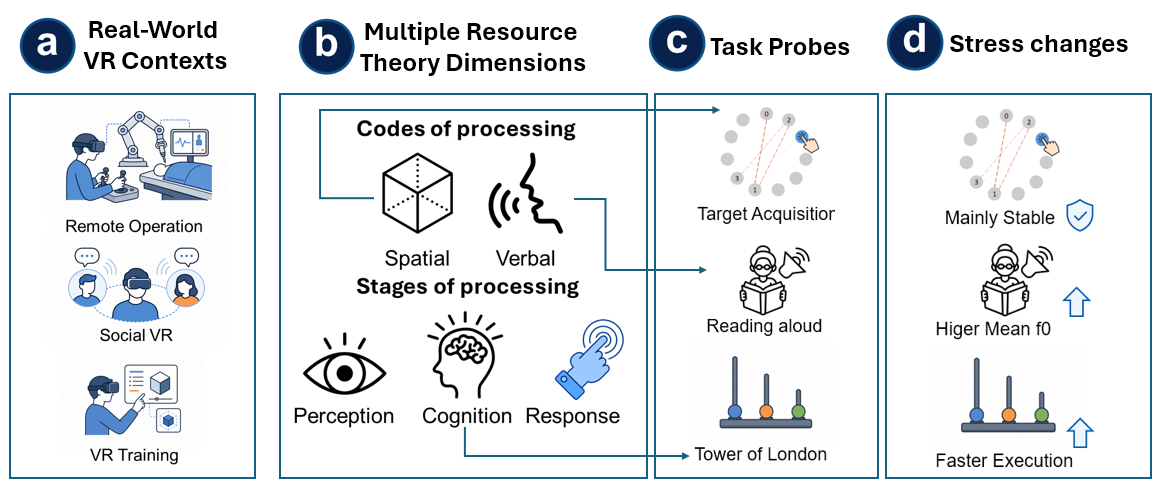
\includegraphics[width=1\textwidth]{Figure/intro.png}
    \caption{Overview of the MRT-informed task-probe approach. We decompose VR interaction demands using selected MRT dimensions and examine stress effects through target acquisition, reading aloud, and Tower of London probes.}
    \label{fig:mrt}
\end{figure*}

\section{Related work}
\label{sec:relatedwork}

\subsection{Situational Impairments and Stress in Interactive Systems}
HCI research has traditionally evaluated interaction techniques under controlled laboratory conditions, often assuming stable cognitive and physical capabilities. Real-world interaction, however, frequently occurs in dynamic contexts that temporarily disrupt these capabilities. \citet{sears2003computers} introduced the concept of situationally induced impairments and disabilities (SIID) to describe such transient limitations in otherwise able-bodied users, arising from contextual factors such as environmental conditions, multitasking, and cognitive demands. Subsequent work has refined SIID as a broad class of context-dependent disruptions affecting interaction across diverse settings~\cite{li2026survey}.

This concept has recently been extended to immersive environments, where perception, action, and feedback are tightly coupled and interaction is therefore especially sensitive to contextual variation~\cite{li2026survey}. Walking and physical encumbrance reduce interaction accuracy and movement efficiency~\cite{li2025weight}, while ambient noise~\cite{li2025estimating} and lighting conditions~\cite{liu2025understanding} affect text entry, pointing performance, and task completion time. These findings indicate that behaviour observed under controlled conditions may not generalize to real-world immersive use.

Beyond environmental and physical factors, situational contexts can induce cognitive disruptions that substantially shape interaction. Acute stress, in particular, has been shown to alter attentional control~\cite{sarsenbayeva2019measuring}, cognitive load~\cite{hou2025cognitive}, and task strategies~\cite{mcguire2023stress}. Within HCI, \citet{sarsenbayeva2019measuring} demonstrated that acute stress affects mobile target acquisition, visual search, and text entry, reducing both accuracy and completion time. Complementary work in affective HCI and motor control suggests that emotional states can modulate low-level motor behaviour: affective priming influences pointing performance under Fitts' Law paradigms~\cite{joo2026quantifying}, and anxiety or cognitive stress can alter physiological tremor and fine motor variability~\cite{budini2022mental}. This line of work, however, focuses on affective priming or single-task motor performance rather than acute social stress in immersive multi-task settings. Taken together, prior work~\cite{sarsenbayeva2019measuring, joo2026quantifying, budini2022mental} establishes that situational and affective states can influence interaction, yet how acute stress manifests in immersive environments across tasks with different cognitive and perceptual demands remains unclear.

\subsection{Inducing and Measuring Stress in Immersive Environments}
A substantial body of research has examined the effects of acute stress on cognition, showing that it impairs working memory, reduces cognitive flexibility, and disrupts executive functioning~\cite{arnsten2009stress,starcke2016effects}, as well as higher-order processes such as decision making and attentional control~\cite{qin2009acute, starcke2012decision}. Thus, stress introduces systematic changes across cognitive functions that are essential for interactive behaviour.

The Trier Social Stress Test (TSST)~\cite{kirschbaum1993trier} is one of the most widely used paradigms for inducing acute stress in controlled settings. By combining public speaking and mental arithmetic calculations under social evaluation, it reliably elicits both physiological and psychological responses. In HCI, the TSST has been used to examine stress effects on mobile interaction, with measurable impacts on target acquisition, visual search, and text entry~\cite{sarsenbayeva2019measuring}, and on reliance decisions during interaction with automated systems~\cite{mcguire2023stress}.

Immersive environments have emerged as a complementary platform for studying stress and emotion. \citet{liszio2018relaxing, liszio2019interactive} showed that VR can both induce and regulate stress, with effects comparable to real-world TSST paradigms. Building on this, \citet{zhang2026seconds} designed a VR-based stress inoculation training system for novice physicians, identifying support strategies such as self-regulation aids, procedure guidance, and sensory support. While that work targets intervention design in a medical training scenario, our study examines how acute stress affects underlying VR interaction components, which can in turn inform when and what kinds of support are needed. Related VR affective computing research further shows that immersive scenes can elicit emotions~\cite{jiang2024immersive} and that interaction itself can modulate emotional experience~\cite{kuang2026understanding}, supporting VR as a controlled yet ecologically relevant platform for studying how stress- and emotion-related state changes unfold during interaction.

Stress is typically assessed through a combination of subjective, physiological, and behavioural measures, including self-report scales such as the State-Trait Anxiety Inventory (STAI)~\cite{spielberger1971state}, heart rate and heart-rate variability~\cite{kim2018stress}, and behavioural indicators such as completion time and error rate~\cite{li2026survey,sarsenbayeva2019measuring}. Together, these measures capture both internal state changes and their observable interaction consequences. Most existing studies, however, focus on a single task context or non-immersive settings, leaving open how stress-induced state changes translate across different interaction modalities within the same immersive environment. 

\subsection{Task-Based Probes and Multiple Resource Theory}
Understanding how stress affects interaction requires tasks that engage different combinations of cognitive, perceptual, and response resources. Multiple Resource Theory (MRT)~\cite{wickens2008multiple} provides a widely used framework for modelling human performance, proposing that interference and workload depend on the degree to which tasks draw on overlapping resource dimensions. MRT organises resources along three primary dimensions: processing stages (perception, cognition, and responding), perceptual modalities (primarily visual and auditory), and processing codes (spatial and verbal); Wickens' 2008 formulation~\cite{wickens2008multiple} further nests focal and ambient visual processing within the visual modality. MRT has therefore been used extensively to reason about why tasks with different resource-demand profiles exhibit different levels of interference, workload, and performance vulnerability. This perspective is well suited to our study because target acquisition task, reading aloud task, and Tower of London task all occur within the same embodied VR setting, yet differ in their dominant resource demands: visuomotor control, verbal delivery, and executive spatial planning, respectively.

In HCI, task-based evaluation is commonly used to probe interaction performance across levels of complexity, including low-level perceptual--motor tasks such as target acquisition~\cite{fitts1964information,li2025estimating,li2025weight}, language-related tasks such as text entry~\cite{mackenzie2003phrase,sarsenbayeva2019measuring} and reading aloud~\cite{dillon2021real}, and higher-level cognitive tasks involving planning and problem solving~\cite{shallice1982specific,banakou2018virtually}. These tasks serve as controlled probes for isolating specific aspects of user performance. Recent work has further shown that different interaction tasks impose distinct cognitive demands that can be characterized using multimodal signals in immersive settings~\cite{hou2025cognitive}. However, such approaches primarily aim to identify task differences or estimate cognitive load, rather than to examine how a situational factor such as stress differentially affects performance across tasks. Prior work on stress and interaction, in turn, has typically treated performance as a single outcome, implicitly assuming uniform degradation under stress.

In this work, we adopt MRT as a task-selection framework to compare interaction performance across tasks with distinct resource profiles. Rather than directly measuring resource competition, we use task-based probes to examine how acute stress affects performance across perceptual -- motor, verbal, and higher-level cognitive domains. This multi-task perspective allows us to move beyond uniform-degradation assumptions and systematically investigate whether stress effects are task-dependent in immersive interaction contexts.


\section{Method}


\begin{figure}[t]
    \centering
    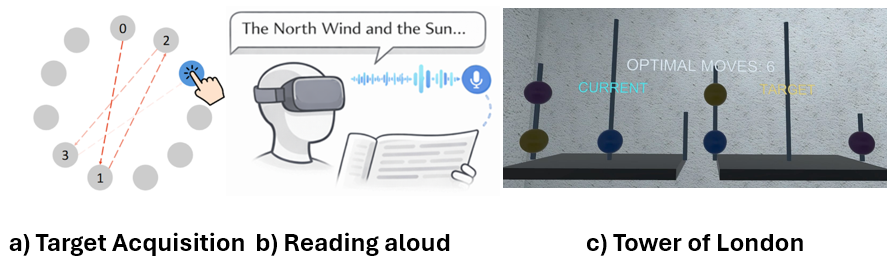
\includegraphics[width=1\linewidth]{Figure/try.png}
    \caption{The tasks used in the experiment: (a) target acquisition; (b) reading aloud; and (c) Tower of London (in-situ VR screenshot).}
    \label{fig:tasks}
\end{figure}
To investigate how acute stress affects different forms of interaction in VR, we implemented three tasks: \textit{target acquisition}, \textit{reading aloud}, and \textit{Tower of London} in a unified immersive environment (~\autoref{fig:tasks}). All tasks were developed in Unity 2022.3.62f3 and deployed on a Meta Quest Pro headset using optical hand tracking (XR Hands) for controller-free interaction. We recorded physiological data with a Polar H10 chest strap.

\subsection{Tasks}
As outlined in Section~\ref{sec:relatedwork}, we used MRT~\cite{wickens2008multiple} as a task-selection framework, rather than as a direct test of resource competition. The three tasks were chosen to sample different combinations of perceptual modality, processing code, response form, and central/executive demand:

\begin{itemize}
    \item \textbf{Target acquisition}: a visual-spatial task with manual response, emphasizing visuomotor coordination and fine motor control with low central planning demands.
    \item \textbf{Reading aloud}: a visual-verbal task with vocal response, emphasizing verbal encoding and speech production under controlled linguistic content.
    \item \textbf{Tower of London}: a visual-spatial task with manual response and substantial central/executive demands, emphasizing sequential planning.
\end{itemize}

Participants performed all tasks while standing, using hand tracking for direct manipulation of virtual objects. Before the experiment, they completed training trials for each task until comfortable with the interaction techniques. Task order was counterbalanced across participants using a Latin square design.

\subsubsection{Target Acquisition Task}
We implemented a target acquisition task using direct hand selection, following the methodology described in ISO 9241-411 for evaluating pointing devices. Eleven spherical targets were arranged in a circular layout 49~cm in front of the participant~\cite{li2025weight}. We instructed participants to select the highlighted targets in a displayed sequence as quickly and as accurately as possible by directly touching each sphere with their index finger. Each round comprised 11 successful selections, with a selection registered when the fingertip entered the 3~cm radius of the target.

To minimise ambiguity, the first target in each sequence was explicitly highlighted and the upcoming target was indicated in advance using a lighter shade. Upon successful selection, the system updated the highlighting to reflect the next target. A cross marker was placed at the centre of each target to indicate the intended selection point and reduce spatial uncertainty. For perceptual clarity and accessibility, all targets were rendered in blue tones, with active and upcoming targets differentiated through luminance rather than hue, avoiding reliance on red-green contrasts.

\subsubsection{Target Acquisition Measures}
We recorded standard pointing performance metrics: movement time, throughput, and endpoint offset, following established evaluation methods~\cite{liu2025understanding}. Movement time (MT) was defined as the elapsed time between consecutive successful selections. Throughput (TP) was computed as a standard Fitts' law efficiency measure:
\[
TP = \frac{ID_e}{MT},
\]
where $ID_e$ is the effective index of difficulty. Endpoint offset was computed as the Euclidean distance between the fingertip and the target centre at the moment of selection:
\[
Offset = \sqrt{(x_f-x_c)^2 + (y_f-y_c)^2 + (z_f-z_c)^2}.
\]
Together, these metrics capture acquisition speed, the speed-accuracy trade-off, and endpoint precision.

We additionally conducted an exploratory trajectory-based analysis of terminal pointing stability. For each successful trial, we computed the fingertip-to-target offset over the final five samples preceding selection and quantified pre-hit stability as their standard deviation:
\[
PreHitStability = \mathrm{SD}(offset_{t-4}, \dots, offset_t).
\]
Lower values indicate more stable endpoint behaviour immediately before acquisition. This measure captures fine-grained terminal variability that may not surface in aggregate outcomes. Prior motor-control work shows that mental calculation can increase postural hand tremor while leaving goal-directed kinetic tremor comparatively unchanged~\cite{budini2022mental}; we therefore treated pre-hit stability as an exploratory indicator of terminal endpoint control rather than as a direct measure of tremor.

\subsubsection{Reading Aloud Task}
We chose reading aloud rather than spontaneous speech as a task to maintain comparable linguistic content across participants and phases while still capturing stress-related changes in vocal production. Participants read excerpts from three phonetically balanced passages widely used in speech research: \textit{The North Wind and the Sun}~\cite{international1999handbook}, \textit{The Rainbow Passage}~\cite{van1972speech}, and the \textit{Grandfather Passage}~\cite{fairbanks1940voice}. To reduce passage-specific repetition and ordering effects, one passage was assigned to each experimental round using random selection without replacement, so that each participant read all three passages exactly once across the three rounds.

For experimental consistency, the passages were trimmed to approximately 110 words while preserving complete sentences, and were selected to have similar Flesch-Kincaid~\cite{kincaid1975derivation} grade levels (6.94, 7.22, and 8.16), indicating broadly comparable reading difficulty. This ensured comparable reading duration across trials while maintaining natural linguistic structure. Passages were displayed as floating text panels in the VR environment, and participants were instructed to read clearly and naturally. Audio and task timestamps were recorded for subsequent analysis.

\subsubsection{Reading Aloud Measures}
We report reading duration, mean fundamental frequency (F0), speech rate, and active speech ratio. To reduce onset hesitation and recording-start artefacts, the first 3~seconds of each recording were excluded from acoustic analysis. Reading duration served as a coarse temporal measure of task completion, while mean F0, speech rate, and active speech ratio were extracted as acoustic indicators of vocal arousal and temporal speech behaviour, following prior work in which speech-based stress and affect analysis commonly relies on prosodic and temporal features~\cite{schewski2025measuring,kappen2022acoustic}.

\subsubsection{Tower of London Task}
We implemented a VR version of the Tower of London (ToL) task~\cite{shallice1982specific} to assess executive planning and sequential problem solving. Participants were presented with an initial arrangement of coloured balls across three pegs together with a target configuration shown nearby, and were instructed to reproduce the target configuration by moving balls between pegs, subject to the constraints that only one ball could be moved at a time and that pegs had limited capacity. Participants manipulated the balls using a pinch gesture~\cite{mikkelsen2025dof}, enabling embodied interaction without controllers. The Unity application logged object states, hand-tracking events from XR Hands, move sequences, and timestamps throughout the task. Each board contained three coloured balls (8~cm in diameter) and three pegs with capacities of three, two, and one ball; adjacent peg centres were separated by 25~cm, and the current and target boards were positioned approximately 60~cm apart. 

To ensure consistent difficulty across rounds,the coloured balls and the pegs shows in random sequence and we used ToL problems with a uniform solution depth of six moves with one rollback structure across rounds, as problem difficulty in the Tower of London is known to depend on both minimum solution length and structural characteristics of the problem~\cite{kaller2004impact}. This design avoided ceiling effects from overly simple problems and floor effects or disproportionate variability from excessively difficult ones~\cite{kaller2012assessing}. 

To minimise direct learning of specific configurations, we varied the spatial arrangement of balls and pegs across rounds while preserving structural difficulty, so participants encountered different instantiations rather than repeating identical layouts. This decision was also informed by pilot testing: with more repeated ToL rounds, repeated exposure substantially reduced errors over time, suggesting that learning effects could overshadow stress-related differences.

\subsubsection{Tower of London Measures}
We report first-move latency, move count, total duration, and execution time. First-move latency was defined as the interval from trial onset to the initiation of the first move, capturing the period during which participants inspected the initial and target configurations and formulated an initial plan~\cite{shallice1982specific}. Move count was the total number of moves required to reach the target configuration, with deviations from the minimum indicating less efficient planning~\cite{kaller2012assessing}. Total duration captured the time taken to complete the entire task~\cite{kaller2012assessing}, and execution time was computed as the difference between total duration and first-move latency, isolating the post-planning execution phase.

\subsection{Procedure}

\subsubsection{Participants}
We recruited 26 participants from the university community. The final analysis included 24 participants (11 female, 13 male) after excluding two with Polar H10 recordings missing. Participants ranged in age from 20 to 31 years ($M = 24.8$, $SD = 3.0$), all reported normal or corrected-to-normal vision and no known motor impairments, and came from a range of disciplines including computer science, nursing, health, design, digital media, and psychology. The sample size is consistent with commonly adopted local standards in HCI experimental studies~\cite{caine2016local}, and recruitment with nearly equal number of male and female participants to avoid gender bias~\cite{van2009stress}.The study was approved by our institutional ethics committee, and all participants provided informed consent prior to the experiment.
\begin{figure*}[!t]
    \centering
    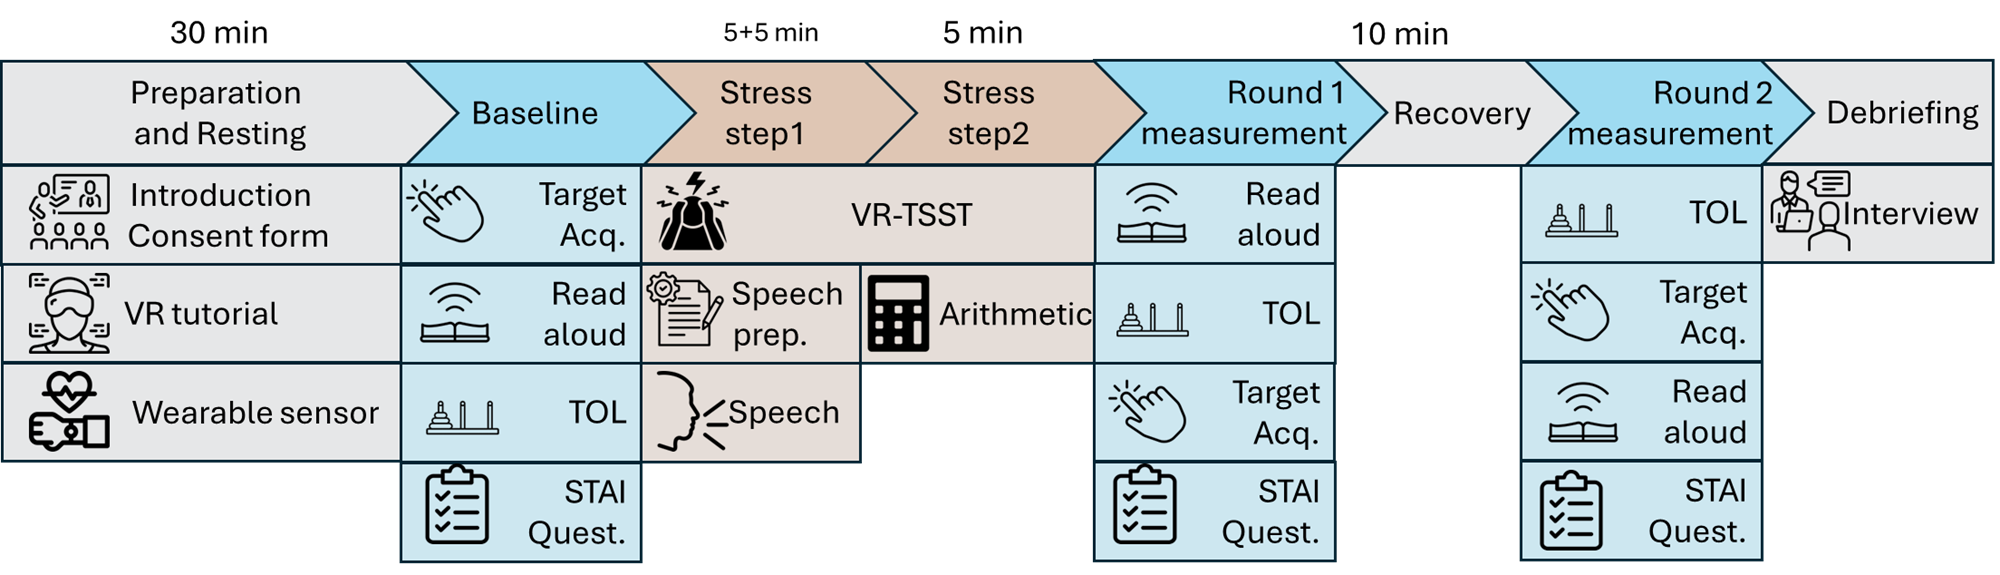
\includegraphics[width=1\textwidth]{Figure/overview.png}
    \caption{Experimental procedure. Abbreviations in the figure: Target Acq. = target acquisition; Speech prep. = speech preparation; Quest. = questionnaire.}
    \label{fig:procedure}
\end{figure*}

To induce stress, we adopted a VR adaptation of the Trier Social Stress Test (VR-TSST). The session comprised four stages: 1) briefing and training, 2) baseline, stress induction with post-stress measurement, and recovery---and lasted approximately 60--70~minutes per participant. An overview is shown in~\autoref{fig:procedure}.

\subsubsection{Preparation and Training}
The experiment took place in the human-centred computing laboratory of our institution. Upon arrival, participants were fitted with a Polar H10 chest strap for physiological data collection. Before fitting the strap, the electrode areas were moistened to improve skin contact, and the strap was positioned around the participant's chest according to the manufacturer's placement guidelines. The sensor was connected via Bluetooth to the recording application, which continuously logged heart-rate estimates and RR intervals throughout the experiment. We first introduced participants to the VR system and they completed a tutorial in which they practised direct finger selection for target acquisition task and pinch gestures for the ToL task. They also rehearsed the ToL rules using a simple example problem and were given a short rest before the formal study began.


\subsubsection{Resting period}
We then left participants alone for 20~minutes to rest and stabilise. During this time we provided them with neutral reading material to keep them occupied without inducing anxiety, as recommended in the TSST protocol~\cite{kirschbaum1993trier}. They subsequently completed the three VR tasks and filled in the STAI-S questionnaire~\cite{spielberger1971state}.

\subsubsection{Stress Induction}
Participants then completed the VR-TSST and were informed that their performance would be video-recorded and reviewed by judges trained in public speaking. They were given 5~minutes to prepare a speech explaining why they would be a suitable candidate for their ideal job, followed by 5~minutes delivering the speech in front of a virtual three-member evaluation committee. Throughout preparation and delivery, the virtual committee members remained present as socially evaluative observers and provided no supportive or encouraging feedback.

Immediately after the speech, participants performed a mental arithmetic task in which they repeatedly subtracted 13 from 1022 and spoke the number sequence aloud~\cite{kirschbaum1993trier}. The same virtual committee remained present throughout, sustaining the socially evaluative atmosphere. Incorrect answers required participants to restart the calculation from the beginning. The subtraction task lasted 5~minutes.

\subsubsection{Post-Stress Measurement (Round 1)}
Immediately after stress induction, participants completed the first post-stress measurement round, again performing the three VR tasks and filling in the STAI questionnaire. Task order differed from the baseline stage to reduce learning effects.

\subsubsection{Recovery and Post-Recovery Measurement (Round 2)}
Following the stress elicitation round, participants were given a 10~minute recovery period. To improve comfort and reduce headset fatigue, they need to remove the headset and rest quietly. After recovery, participants completed the second measurement round and filled in the STAI questionnaire.

\subsubsection{Participant Debriefing}
Finally, we debriefed participants about the study, explained that experiencing stress during the experiment was expected, and clarified that the tasks were intentionally demanding and did not reflect participants' aptitude or ability. We also informed them that their performance had not been evaluated by a real judging panel. We then conducted a short semi-structured interview, asking participants to report their subjective perception of the experiment and the effect of stress on their performance.
\subsection{Stress Validation Measures}
We validated stress occurrence using participants' self-reported anxiety and physiological responses. We measured self-reported anxiety with the state scale of the State-Trait Anxiety Inventory – State scale (STAI-S) after each round~\cite{spielberger1971state}. We recorded physiological responses  with a Polar H10 chest strap. To calculate high-frequency heart rate variability (HF HRV), a frequency-domain measure of heart rate variability (HRV),we extracted heart rate and inter-beat interval (IBI) estimates derived from the RR intervals. Following prior work~\cite{sarsenbayeva2019measuring}, We ordered IBI samples by timestamp, interpolated them to a uniformly sampled 4~Hz time series, and analysed using an Fast Fourier Transform (FFT)-based sliding-window procedure. For each 512-sample window, we computed the frequency spectrum and summed spectral magnitude within the high-frequency band (HF HRV: 0.15--0.40~Hz). HF HRV values were averaged within each physiological analysis window and log-transformed before statistical analysis. In addition to HF HRV, we computed mean heart rate (HR) and the standard deviation of normal-to-normal intervals (SDNN) as indicators of cardiovascular arousal. Although the root mean square of successive differences between normal heartbeats (RMSSD) is often used as an index of parasympathetic activity, the VR-TSST in our study involved continuous speech and aloud arithmetic tasks, which may directly affect short-term beat-to-beat variability. We therefore use SDNN as the primary time-domain HRV measure and treat RMSSD as a complementary measure~\cite{shaffer2017overview}. All physiological data processing and statistical analyses were conducted in Python using custom scripts with pandas, NumPy, SciPy, and Matplotlib.




\section{Results}

\subsection{Stress Validation}
\label{sec:stress-validation}
We first examined whether the VR-TSST successfully induced stress, analysing STAI-S, mean HR, SDNN, and log-transformed HF HRV across the three phases. For each stress-validation measure, we used a one-way repeated-measures ANOVA to test the overall effect of phase, followed by pairwise comparisons between adjacent phases. Pairwise $p$ values were Bonferroni-adjusted across the three phase comparisons for each measure. STAI-S values are reported as scale scores, mean HR in beats per minute (bpm), SDNN in milliseconds (ms), and HF HRV as log-transformed high-frequency spectral power.

STAI-S state scores (~\autoref{fig:hr}-a) showed a significant effect of phase, $F(2,46)=25.77, p<.001$. Self-reported anxiety rose sharply from Baseline ($M=32.38$, $SD=7.83$) to Post-Stress ($M=47.58$, $SD=10.29$; $p<.001$) and then declined at Post-Recovery ($M=35.25$, $SD=11.58$; Post-Stress vs.\ Post-Recovery: $p<.001$), with no significant difference between Baseline and Post-Recovery ($p=.231$). The protocol therefore successfully elevated subjective anxiety during stress induction. The effect was large, $\eta_p^2=.528$; anxiety increased by 15.21 points from Baseline to Post-Stress, 95\% CI $[10.52, 19.89]$.

Mean HR (~\autoref{fig:hr}-b) likewise showed a significant phase effect, $F(2,46)=31.12, p<.001$, increasing from Baseline ($M=88.10$~bpm, $SD=9.03$~bpm) to Stress Induction ($M=92.13$~bpm, $SD=10.62$; $p<.001$) and decreasing at Post-Recovery ($M=83.85$~bpm, $SD=8.41$; Stress Induction vs.\ Post-Recovery: $p<.001$). Baseline and Post-Recovery also differed significantly ($p<.001$), indicating a substantial reduction in physiological arousal after the stress period. The effect was large, $\eta_p^2=.575$; heart rate increased by 4.03~bpm from Baseline to Stress Induction, 95\% CI $[2.06, 6.01]$.

For comparison with prior stress-interaction work, we also examined frequency-domain HF HRV (~\autoref{fig:hr}-c). Log-transformed HF HRV showed a significant effect of phase, $F(2,46)=3.60, p=.035$. The Baseline-to-Stress decrease did not reach significance (Baseline: $M=10.60$, $SD=0.87$; Stress Induction: $M=10.42$, $SD=0.72$; $p=.128$), but HF HRV increased significantly from Stress Induction to Post-Recovery ($M=10.69$, $SD=0.76$; $p=.017$). The effect was moderate, $\eta_p^2=.135$; the Baseline-to-Stress change was $-0.18$, 95\% CI $[-0.42, +0.06]$, and the Stress to Post-Recovery change was $+0.27$, 95\% CI $[+0.05, +0.48]$.

SDNN (~\autoref{fig:hr}-d) showed a significant phase effect, $F(2,46)=8.57, p<.001$, decreasing from Baseline ($M=71.89$~ms, $SD=32.83$) to Stress Induction ($M=56.96$~ms, $SD=19.99$; $p=.005$) and rising again at Post-Recovery ($M=73.31$~ms, $SD=23.47$; $p<.001$). Baseline and Post-Recovery did not differ significantly ($p=.729$). Because lower SDNN reflects reduced HRV and elevated arousal, this pattern provides further evidence that stress induction altered participants' physiological state. The effect was large, $\eta_p^2=.272$; SDNN decreased by 14.93~ms from Baseline to Stress Induction, 95\% CI $[-24.95, -4.91]$, and increased by 16.35~ms from Stress Induction to Post-Recovery, 95\% CI $[+7.69, +25.01]$.

Together, the STAI, HR, and HRV results confirm that the stress-induction protocol elevated both subjective anxiety and physiological arousal. ~\autoref{tab:all-change-summary} summarises the direction and magnitude of percentage change between adjacent phases for ease of comparison.

% \subsection{Validation of Stress Occurrence}

% We first examined whether the VR-TSST successfully induced stress. We analysed STAI-S, mean HR, SDNN, and log-transformed HF HRV across phases. 

% STAI state scores showed a statistically significant effect of phase, $F(2,46)=25.77, p<.001$. Participants reported significantly higher anxiety after stress induction (Baseline: $M=32.38$, $SD=7.83$; Post-Stress: $M=47.58$, $SD=10.29$; Baseline vs.\ Post-Stress: $p<.001$), followed by a significant decrease during Recovery (Recovery: $M=35.25$, $SD=11.58$; Post-Stress vs.\ Recovery: $p<.001$). No significant difference was observed between Baseline and Recovery ($p=.231$). These result shows in ~\autoref{fig:stai} indicate that the protocol successfully increased subjective anxiety during the stress-induction phase.


% Mean HR shows in ~\autoref{fig:hr} also showed a statistically significant effect of phase, $F(2,46)=31.12, p<.001$. Mean HR increased from Baseline ($M=88.10$ bpm, $SD=9.03$) to Stress Induction ($M=92.13$ bpm, $SD=10.62$; Baseline vs.\ Stress Induction: $p<.001$), and significantly decreased during Post-stress Recovery ($M=83.85$ bpm, $SD=8.41$; Stress Induction vs.\ Post-stress Recovery: $p<.001$). Baseline and Recovery also differed significantly ($p<.001$), indicating a substantial reduction in physiological arousal after the stress period.

% We further examined HRV using SDNN. SDNN in ~\autoref{fig:sdnn} showed a significant phase effect, $F(2,42)=8.35, p<.001$. SDNN decreased from Baseline ($M=72.58$ ms, $SD=34.27$) to Stress Induction ($M=57.56$ ms, $SD=21.75$; Baseline vs.\ Stress Induction: $p=.006$), and increased during Post-stress Recovery ($M=73.50$ ms, $SD=22.59$; Stress Induction vs.\ Post-stress Recovery: $p=.001$). Baseline and Recovery did not significantly differ ($p=.819$). Since lower SDNN values indicate reduced HRV and elevated physiological arousal, these results provide further evidence that the stress induction successfully altered participants' physiological state.


% For comparison with prior stress-interaction work, we also examined frequency-domain HF HRV~\ref{fig:hrv_fft}. The repeated-measures ANOVA on log-transformed HF HRV showed a statistically significant effect of phase, $F(2,42)=3.28, p=.047$. Although the decrease from Baseline to Stress Induction did not reach significance (Baseline: $M=10.57$, $SD=0.89$; Stress Induction: $M=10.40$, $SD=0.75$; $p=.122$), HF HRV significantly increased from Stress Induction to Post-stress Recovery (Recovery: $M=10.64$, $SD=0.76$; $p=.017$). 
% Together, the STAI, HR, and HRV results indicate that the stress-induction protocol successfully increased both subjective anxiety and physiological arousal. For ease of comparison across validation measures, ~\autoref{tab:validation-change} summarises the direction and magnitude of percentage changes between adjacent phases.
\begin{figure*}[t]
\centering
\begin{subfigure}[t]{0.24\textwidth}
    \centering
    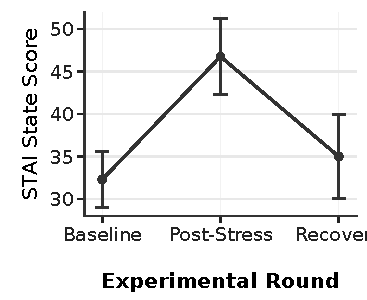
\includegraphics[width=\linewidth]{Figure/stress_stai.pdf}
    \caption{STAI-S}
    \label{fig:stress-stai}
\end{subfigure}\hfill
\begin{subfigure}[t]{0.24\textwidth}
    \centering
    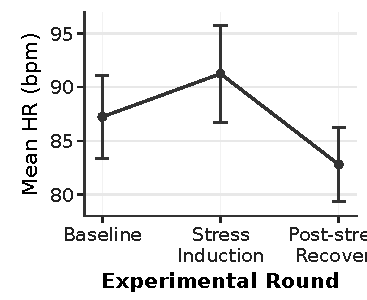
\includegraphics[width=\linewidth]{Figure/stress_hr.pdf}
    \caption{Mean Heart Rate}
    \label{fig:stress-hr}
\end{subfigure}\hfill
\begin{subfigure}[t]{0.24\textwidth}
    \centering
    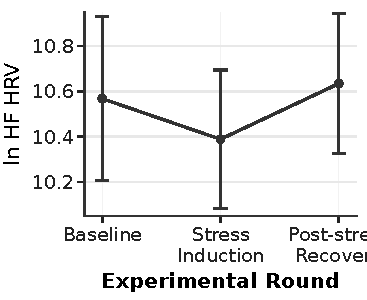
\includegraphics[width=\linewidth]{Figure/stress_hfhrv.pdf}
    \caption{HF HRV}
    \label{fig:stress-hfhrv}
\end{subfigure}\hfill
\begin{subfigure}[t]{0.24\textwidth}
    \centering
    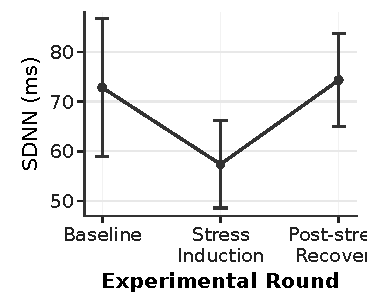
\includegraphics[width=\linewidth]{Figure/stress_sdnn.pdf}
    \caption{SDNN}
    \label{fig:stress-sdnn}
\end{subfigure}

\caption{Validation of stress induction using subjective anxiety and physiological measures. Error bars show 95\% confidence intervals.}
\label{fig:hr}
\end{figure*}

\subsection{Target Acquisition Task}
We next examined target acquisition task performance using mean acquisition time, Fitts' throughput, and spatial offset. One-way repeated-measures ANOVAs showed no significant effect of phase on acquisition time ($F(2,46)=0.10, p=.907$), throughput ($F(2,46)=0.09, p=.912$), or offset ($F(2,46)=0.35, p=.708$), and pairwise comparisons revealed no significant differences between any pair of phases (all $p>.05$). All three effects were negligible in size ($\eta_p^2=.004$, $.004$, and $.015$ for acquisition time, throughput, and offset respectively). Between Baseline and Post-Stress, acquisition time differed by $+17.67$~ms, 95\% CI $[-93.93, +129.26]$; throughput by $-0.02$~bit/s, 95\% CI $[-0.36, +0.33]$; and offset by $+0.05$~cm, 95\% CI $[-0.05, +0.15]$.

Beyond these predefined metrics, we conducted an exploratory analysis of terminal pointing stability, defined as the standard deviation of the finger-to-target-centre offset across the final five samples before successful selection (lower values indicate more stable terminal movements). Mean pre-hit variability (~\autoref{fig:tara}-a) decreased from Baseline ($M=0.341$) to Post-Stress ($M=0.275$) and rose again at Post-Recovery ($M=0.323$). The overall phase effect did not reach significance ($p=.127$), but pairwise comparisons indicated a significant decrease from Baseline to Post-Stress ($p=.025$) and a significant increase from Post-Stress to Post-Recovery ($p=.049$). This suggests that terminal hand movements may have become more stable during the stress phase, even though conventional endpoint measures showed no significant change. ~\autoref{tab:all-change-summary} summarises the phase-wise direction and magnitude of change across target acquisition measures,\autoref{tab:all-change-summary} summarises the observed phase-wise changes in the predefined target acquisition measures and the exploratory pre-hit variability measure.

% \subsubsection{Target Acquisition}

% We then investigated the effect of stress on target acquisition performance using mean target acquisition time, Fitts' throughput, and spatial offset size. A one-way repeated-measures ANOVA showed no statistically significant effect of phase on target acquisition time ($F(2,46)=0.10, p=.907$), throughput ($F(2,46)=0.09, p=.912$), or offset size ($F(2,46)=0.35, p=.708$). Pairwise comparisons also revealed no statistically significant differences between Baseline and Post-Stress or between Post-Stress and Recovery for any of these measures (all $p>.05$). These results indicate that stress induction did not significantly affect target acquisition speed, throughput, or endpoint accuracy in our XR task.

% Beyond the predefined target acquisition metrics, we also conducted an exploratory analysis of terminal pointing stability using the standard deviation of the finger-to-target-center offset during the final five pre-hit samples before successful selection. Lower values indicate more stable hand movements immediately before target acquisition. Mean pre-hit offset variability in ~\autoref{fig:std} decreased from Baseline ($M=0.341$) to Post-Stress ($M=0.275$), and then increased again during Recovery ($M=0.323$). Although the overall phase effect did not reach significance ($p=.127$), pairwise comparisons indicated a significant decrease from Baseline to Post-Stress ($p=.025$) and a significant increase from Post-Stress to Recovery ($p=.049$). This suggests that terminal hand movements may have become more stable during the stress phase, even though conventional endpoint offset measures did not show significant changes. ~\autoref{tab:ta-change} provides a compact summary of the phase-wise direction and magnitude of change across target acquisition measures, highlighting the contrast between stable predefined outcomes and the exploratory terminal stability metric.




\begin{figure}[t]
\centering
\begin{subfigure}[t]{0.48\columnwidth}
    \centering
    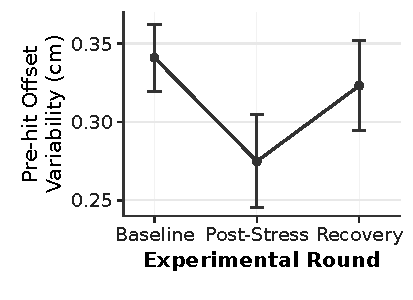
\includegraphics[width=\linewidth]{Figure/prehit_stability.pdf}
    \caption{Exploratory terminal pointing stability}
    \label{fig:prehit-stability}
\end{subfigure}\hfill
\begin{subfigure}[t]{0.48\columnwidth}
    \centering
    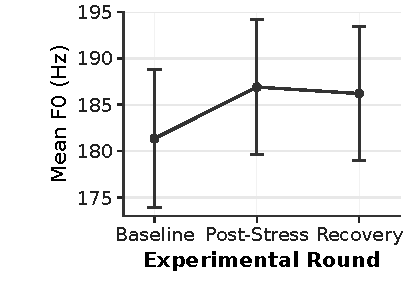
\includegraphics[width=\linewidth]{Figure/reading_mean_f0.pdf}
    \caption{Reading aloud mean F0}
    \label{fig:reading-f0}
\end{subfigure}

\caption{Stress-related changes in target acquisition task and reading aloud task. Error bars show 95\% confidence intervals.}
\label{fig:tara}
\end{figure}
\subsection{Reading Aloud Task}
We then examined reading aloud performance using reading duration, mean fundamental frequency (F0), speech rate, and active speech ratio. A one-way repeated-measures ANOVA showed a significant effect of phase on mean F0 ($F(2,46)=4.26, p=.020$): F0 was higher in Post-Stress ($M=186.91$~Hz, $SD=35.62$) than in Baseline ($M=181.35$~Hz, $SD=36.36$; $p=.020$), but did not differ significantly between Post-Stress and Post-Recovery ($M=186.20$~Hz, $SD=35.38$; $p=.689$). Reading duration, speech rate, and active speech ratio did not show significant effects of phase (all $p>.05$). Mean values are visualised in ~\autoref{fig:tara}-b, and ~\autoref{tab:all-change-summary} summarises the phase-wise percentage changes across vocal measures. The effect on mean F0 was moderate, $\eta_p^2=.156$; F0 rose by 5.55~Hz from Baseline to Post-Stress, 95\% CI $[+0.96, +10.15]$. The remaining vocal measures showed negligible effects: reading duration $F(2,46)=0.27$, $p=.765$, $\eta_p^2=.012$; speech rate $F(2,46)=0.85$, $p=.432$, $\eta_p^2=.036$; active speech ratio $F(2,46)=0.91$, $p=.409$, $\eta_p^2=.038$.

% \subsubsection{Reading Aloud}

% We next examined the effect of stress on read-aloud performance using reading duration, mean fundamental frequency (F0), speech rate, and active speech ratio. The first 3 seconds of each recording were excluded to reduce onset hesitation and recording-start artifacts. A one-way repeated-measures ANOVA showed a statistically significant effect of phase on mean F0 ($F(2,46)=4.26, p=.020$). Pairwise comparisons indicated that mean F0 was significantly higher in the Post-Stress phase ($M=186.91$ Hz, $SD=35.62$) than in Baseline ($M=181.35$ Hz, $SD=36.36$; $p=.020$). However, no statistically significant difference was observed between Post-Stress and Recovery (Recovery: $M=186.20$ Hz, $SD=35.38$; $p=.689$). In contrast, reading duration, speech rate, and active speech ratio did not show statistically significant effects of phase (all $p>.05$). These results suggest that stress induction altered participants' vocal arousal, while leaving coarse speech timing measures relatively stable. The mean values for read-aloud measures are visualised in ~\autoref{fig:ra}, while ~\autoref{tab:ra-change} summarises the phase-wise percentage changes to facilitate comparison across vocal measures.

\subsection{Tower of London Task}
Finally, we examined ToL task performance using first-move latency, move count, total duration, and execution time.
The repeated-measures ANOVA on total duration were not significant ($F(2,46)=2.50, p=.093$). However, pairwise comparisons showed that total duration(~\autoref{fig:tol}-a) was significantly shorter in Post-Stress ($M=36.22$~s, $SD=16.12$) than in Baseline ($M=51.54$~s, $SD=35.86$; $p=.009$), with no significant difference between Post-Stress and Post-Recovery ($M=43.84$~s, $SD=26.00$; $p=.179$). A similar pattern emerged for execution time (~\autoref{fig:tol}-b): the omnibus test was not significant ($F(2,46)=2.26, p=.116$), but execution time was significantly shorter in Post-Stress ($M=20.51$~s, $SD=13.76$) than in Baseline ($M=34.02$~s, $SD=29.02$; $p=.007$), with no significant difference between Post-Stress and Post-Recovery ($p=.348$). First-move latency and move count showed no significant phase effects (all $p>.05$). Both timing effects were small to moderate in size ($\eta_p^2=.098$ for total duration and $.089$ for execution time). Total duration was 15.32~s shorter in Post-Stress than Baseline, 95\% CI $[-26.51, -4.13]$, and execution time 13.52~s shorter, 95\% CI $[-23.00, -4.04]$. The planning measures showed negligible effects: first-move latency $F(2,46)=0.27$, $p=.767$, $\eta_p^2=.011$; move count $F(2,46)=0.80$, $p=.456$, $\eta_p^2=.034$.

These results indicate that stress induction did not broadly improve ToL planning performance but was associated with faster task execution following stress. This reduction in execution time should be interpreted cautiously, as it may reflect more hurried or urgent execution rather than a genuine enhancement of planning ability. ~\autoref{tab:all-change-summary} summarises the direction and relative magnitude of phase-wise changes across ToL measures, showing that the clearest shifts occurred in total duration and execution time rather than in planning-specific measures.
% \subsubsection{Tower of London}

% We then investigated the effect of stress on Tower of London (ToL) performance using first-move latency, move count, total duration and execution time. Execution time was computed as total task duration minus first-move latency, capturing the time spent executing moves after the initial planning period.

% A one-way repeated-measures ANOVA did not show a statistically significant effect of phase on total duration ($F(2,46)=2.28, p=.114$)~\ref{fig:tol_dur}. However, pairwise comparisons indicated that total duration was significantly shorter in the Post-Stress phase ($M=36.22$ s, $SD=16.12$) than in Baseline ($M=50.87$ s, $SD=36.30$; $p=.013$). No statistically significant difference was observed between Post-Stress and Recovery (Recovery: $M=44.51$ s, $SD=25.58$; $p=.147$).


\begin{figure}[t]
\centering
\begin{subfigure}[t]{0.48\columnwidth}
    \centering
    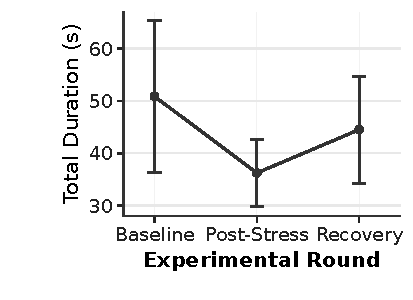
\includegraphics[width=\linewidth]{Figure/tol_total_duration.pdf}
    \caption{Total duration}
    \label{fig:tol-duration}
\end{subfigure}
\begin{subfigure}[t]{0.48\columnwidth}
    \centering
    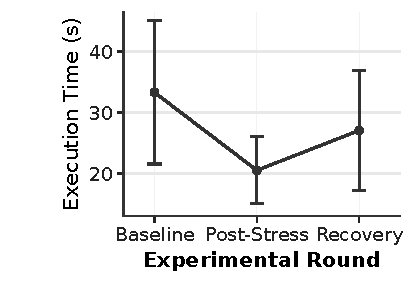
\includegraphics[width=\linewidth]{Figure/tol_execution_time.pdf}
    \caption{Execution time}
    \label{fig:tol-execution}
\end{subfigure}\hfill


\caption{Tower of London timing measures across experimental phases. Error bars show 95\% confidence intervals.}
\label{fig:tol}
\end{figure}
% Similarly, a one-way repeated-measures ANOVA did not show a statistically significant effect of phase on execution time ($F(2,46)=1.98, p=.149$)~\ref{fig:tol_exe}. Nevertheless, pairwise comparisons showed that execution time was significantly shorter in the Post-Stress phase ($M=20.51$ s, $SD=13.76$) than in Baseline ($M=33.29$ s, $SD=29.38$; $p=.010$). No statistically significant difference was found between Post-Stress and Recovery ($p=.295$).

% In contrast, first-move latency and move count did not show statistically significant effects of phase (all $p>.05$). Taken together, these results indicate that stress induction did not broadly improve ToL planning performance, but was associated with faster task execution following stress induction. This reduction in execution time should be interpreted cautiously, as it may reflect faster or more urgent task execution rather than a broad enhancement of planning ability. ~\autoref{tab:tol-change} summarises the direction and relative magnitude of phase-wise changes across Tower of London measures, showing that the clearest shifts were observed in total duration and execution time rather than in planning-specific measures.


\subsection{Participant Feedback}
Post-study interviews suggested that participants did not experience the stress induction in a uniform way. Seven participants reported feeling more focused during the post-stress tasks, whereas three reported little or no noticeable change and four found the change difficult to describe. Participants also differed in which part of the VR-TSST they found most stressful: thirteen identified the mental arithmetic phase as more stressful than the speech phase, while three reported that the speech task felt less stressful because the audience consisted of virtual characters rather than real people. However, this pattern was not universal; one participant reported feeling ashamed during the speech task, and two participants noted that not being able to see their hands during the induction increased their tension in VR.
Several comments were also consistent with the behavioural results. Three participants explicitly stated that, after stress induction, they wanted to complete the subsequent tasks more quickly, which aligns with the shorter execution time observed in the Tower of London task. At the same time, one participant reported feeling calmer after the induction and found the later tasks easier, highlighting individual differences in post-stress responses. Overall, the interviews suggest that the VR-TSST elicited a mixture of heightened pressure, narrowed attention, altered embodiment, and task-focused urgency rather than a single uniform subjective response.

\begin{table}[t]
\centering
\large
\caption{Summary of stress-related changes across validation and task measures. Colored arrows indicate statistically significant pairwise differences ($p < .05$), whereas black arrows denote descriptive but non-significant changes. * denotes an exploratory metric.}
\label{tab:all-change-summary}
\normalsize
\resizebox{\columnwidth}{!}{
\begin{tabular}{lcc}
\toprule
\textbf{Measure} & \textbf{Baseline $\rightarrow$ Post-Stress} & \textbf{Post-Stress $\rightarrow$ Post-Recovery} \\
\midrule

\multicolumn{3}{l}{\textbf{Stress validation}} \\
\quad STAI-S
& \textcolor{orange}{\(\uparrow\) 46.9\%}
& \textcolor{blue}{\(\downarrow\) 25.9\%} \\
\quad Mean HR
& \textcolor{orange}{\(\uparrow\) 4.6\%}
& \textcolor{blue}{\(\downarrow\) 9.0\%} \\
\quad SDNN
& \textcolor{blue}{\(\downarrow\) 20.8\%}
& \textcolor{orange}{\(\uparrow\) 28.7\%} \\
\quad ln HF HRV
& \textcolor{black}{\(\downarrow\) 1.7\%}
& \textcolor{orange}{\(\uparrow\) 2.6\%} \\

\midrule
\multicolumn{3}{l}{\textbf{Target acquisition}} \\
\quad MT
& \textcolor{black}{\(\uparrow\) 2.0\%}
& \textcolor{black}{\(\downarrow\) 2.0\%} \\
\quad Offset
& \textcolor{black}{\(\uparrow\) 2.5\%}
& \textcolor{black}{\(\downarrow\) 0.5\%} \\
\quad TP
& \textcolor{black}{\(\downarrow\) 0.5\%}
& \textcolor{black}{\(\downarrow\) 1.9\%} \\
\quad Pre-hit Stability*
& \textcolor{blue}{\(\downarrow\) 19.4\%}
& \textcolor{orange}{\(\uparrow\) 17.5\%} \\

\midrule
\multicolumn{3}{l}{\textbf{Reading aloud}} \\
\quad Mean F0
& \textcolor{orange}{\(\uparrow\) 3.1\%}
& \textcolor{black}{\(\downarrow\) 0.4\%} \\
\quad Speech Rate
& \textcolor{black}{\(\uparrow\) 1.0\%}
& \textcolor{black}{\(\downarrow\) 3.6\%} \\
\quad Reading Duration
& \textcolor{black}{\(\uparrow\) 1.5\%}
& \textcolor{black}{\(\downarrow\) 2.3\%} \\
\quad Active Speech Ratio
& \textcolor{black}{\(\downarrow\) 0.6\%}
& \textcolor{black}{\(\downarrow\) 3.7\%} \\

\midrule
\multicolumn{3}{l}{\textbf{Tower of London}} \\
\quad First-Move Latency
& \textcolor{black}{\(\downarrow\) 10.6\%}
& \textcolor{black}{\(\uparrow\) 11.1\%} \\
\quad Move Count
& \textcolor{black}{\(\downarrow\) 6.2\%}
& \textcolor{black}{\(\uparrow\) 15.3\%} \\
\quad Total Duration
& \textcolor{blue}{\(\downarrow\) 29.7\%}
& \textcolor{black}{\(\uparrow\) 22.9\%} \\
\quad Execution Time
& \textcolor{blue}{\(\downarrow\) 39.7\%}
& \textcolor{black}{\(\uparrow\) 31.8\%} \\

\bottomrule
\end{tabular}
}
\end{table}
\section{Discussion}

\subsection{Stress as Task-Dependent Behavioural Modulation}
Our goal is not to present a deployed stress-adaptive VR system but to characterise how acute stress changes behaviour across interaction components. The MRT-informed task-probe framing offers an analytical basis for reasoning about stressful VR situations that have not yet been directly studied. By considering the resource-demand profile of the current task, designers can anticipate which aspects of interaction may remain stable and which may require support. Our findings suggest that acute stress in VR should not be treated as a uniform disruptor of interaction in VR. Across the three task probes, stress-related changes appeared selectively across measures rather than as a consistent decline in speed, accuracy, or efficiency.

For the target acquisition task, we did not detect statistically significant phase differences in movement time, throughput, or endpoint offset. These findings do not establish that target acquisition is unaffected by stress. The exploratory pre-hit analysis describes a possible phase-associated change in terminal offset variability that requires further investigation. 
%Exploratory axis-wise analyses further indicated that stress-related changes in endpoint error may be direction-specific rather than isotropic: the vertical component showed a modest increase from \textit{Baseline} measurements to \textit{Post-Stress} although the analysis of overall offset did not detect a statistically significant phase effect. We interpret this cautiously, but it raises the possibility that VR pointing under stress may be modulated by axis-specific factors such as hand-tracking characteristics, posture, or embodied spatial alignment.  

For the reading aloud task, stress effects were more evident in vocal characteristics than in the task itself. Mean F0 increased after stress induction, whereas no statistically significant phase effects were detected in reading duration, speech rate, and active speech ratio remained comparatively stable. Constrained verbal production may therefore preserve coarse temporal structure while still reflecting stress through prosodic arousal.

For the ToL task, stress influenced the total duration and execution time, but did not have no statistics significance on first-move latency and move counts. We do not interpret this as evidence that stress improved planning ability. A more cautious reading is that stress altered execution dynamics after the initial planning period, possibly reflecting a more action-oriented or urgent interaction style. This phenomenon may be consistent with attentional narrowing accounts of stress and arousal, suggesting that stress can bias attention toward immediate task-relevant goals while reducing the breadth of monitoring or deliberation~\cite{easterbrook1959effect}. 
Thus, participants may have completed the ToL task more quickly under stress not because planning improved, but because they shifted toward more immediate, action-oriented execution.

These results indicate that acute stress in immersive environments may manifest less as a consistent global decrement and more as selective behavioural changes across tasks with different resource-demand profiles. This interpretation helps explain why some metrics remained stable while others showed more localised or phase-specific effects. One possible explanation comes from Multiple Resource Theory (MRT)~\cite{wickens2008multiple}, which suggests that performance depends on multiple partially independent resource channels spanning perceptual, cognitive, and response processes. From this perspective, acute stress need not reduce all forms of performance equally: it may instead manifest differently depending on the resource demands of the task. Our results are broadly consistent with such an account. Tasks relying more strongly on higher-level planning showed clearer changes in execution dynamics, perceptual-motor performance remained relatively stable at the level of predefined outcome metrics, and verbal changes were expressed primarily through vocal arousal rather than broad timing disruption. This pattern suggests that stress reshapes interaction differently depending on the resources most relevant to a given task.
\subsection{Practical significance}

\subsection{Implications for Stress-Aware VR Design}
Our findings have several implications for the design of stress-aware immersive systems. Most importantly, stress-aware adaptation in VR should not assume that stress affects all interaction in the same way. Hence, adaptive supports may be more effective when informed by the demands of the current task.

First, stress-aware systems should adapt support to the current task rather than applying a generic stress response. Planning-heavy tasks may benefit from subgoal cues, step previews, or reduced concurrent demands, whereas simple target selection may require little intervention unless fine precision is critical. Second, systems should monitor changes in interaction dynamics, not only overt errors or failures: in our study, several stress-related changes appeared in timing, vocal arousal, or terminal movement dynamics rather than in accuracy. Third, support may need to continue into recovery, since some measures did not immediately return to baseline, suggesting that post-stress interaction may remain altered even after the stressor has ended.

More broadly, these findings point toward opportunities for stress-aware VR systems that integrate user state with task structure. We do not claim to have validated a specific adaptive system. Here, our results suggest that future adaptive immersive systems may benefit from considering not only whether a user is stressed, but also what kind of interaction they are currently performing.

\subsection{Limitations and Future Work}
A first limitation concerns potential learning and order effects.Because phase order was fixed, phase-associated changes cannot be attributed specifically to stress, as practice, fatigue, and familiarisation may also have contributed. Although we used a Latin-square-based ordering strategy and varied the reading aloud passages and ToL configurations across rounds, the repeated-measures design may still have introduced practice-related changes. This issue was considered during pilot testing, where repeated exposure to multiple ToL and target acquisition trials within the same session appeared to amplify familiarity effects, informing our decision to use a more constrained design in the main study with one ToL instance and one target acquisition block per round. Even so, residual practice effects cannot be fully ruled out. Our sample size is comparable to many controlled within-subject HCI studies, but may still limit sensitivity to modest task-specific effects and individual-difference patterns.

A second limitation is that our three tasks were intentionally designed as controlled probes rather than as full end-to-end VR workflows. Although target acquisition, reading aloud, and ToL task allowed us to isolate specific classes of interaction under stress, they do not fully capture the complexity, context switching, or social and semantic richness of real-world VR use. Our findings should therefore be interpreted as evidence about stress-sensitive interaction components rather than as a complete account of stress effects in deployed VR applications.

A third limitation concerns the scope of our MRT-based interpretation. Although the task battery was informed by MRT, the study did not directly test resource competition in the classical MRT sense: we did not employ dual-task or concurrent-task paradigms, nor did we manipulate competing demands within the same trial. Instead, we compared separate task probes that differed in their dominant interaction demands. MRT should therefore be understood here as a task-selection and interpretive lens, rather than as a theory directly validated by our experimental design.

A final limitation is that TSST induction is unlikely to operate as a uniform stress dose across individuals. Prior work suggests that responses to the TSST may depend on participant-specific factors such as ability, engagement, and coping style~\cite{kudielka2007ten}, which is especially relevant in the arithmetic phase, where participants may differ in response speed, accuracy, and how they react to errors or interruptions. One advantage of VR is that such induction-phase behaviour can be both tightly controlled and continuously logged. We explored whether arithmetic-phase dynamics were associated with downstream task changes, but did not observe robust significant relationships in the current sample. Future work should examine these individual-difference effects more systematically with larger samples. Our participants were young adults recruited from a university population, so the findings may not generalise to older users or to individuals with cognitive impairment, elevated baseline anxiety, anxiety-related conditions, or other psychosocial factors that could influence stress reactivity and interaction performance.




\section{Conclusion}
We investigated how acute stress affects interaction in immersive VR across components with distinct cognitive and perceptual demands. Drawing on Multiple Resource Theory as a task-selection framework, we examined three controlled probes within a unified VR environment, target acquisition, reading aloud, and ToL task, under a VR adaptation of the Trier Social Stress Test, combining behavioural performance, speech features, and physiological responses with self-reported anxiety.

Our results do not support a uniform-degradation account of stress in VR. Predefined target acquisition task outcomes remained broadly stable, while an exploratory measure of terminal pointing stability suggested subtler changes in fine-grained endpoint control. Reading aloud showed elevated mean F0 with comparatively stable timing, indicating that constrained verbal production preserves coarse temporal structure while still reflecting prosodic arousal. ToL task showed shorter total duration and execution time after stress, without corresponding changes in first-move latency or move count, suggesting altered execution dynamics rather than improved planning. Together, these patterns indicate that stress in VR manifests as selective, task-dependent behavioural modulation rather than as a single global decrement.

These findings extend situational-impairment research to immersive environments and offer an MRT-informed task-probe framing for reasoning about stress-related SIID in complex VR tasks. They also carry concrete design implications: stress-aware VR systems should adapt support to the current task rather than apply a generic response, monitor interaction dynamics beyond overt errors, and consider that post-stress effects may persist into recovery. More broadly, our work points toward stress-aware immersive systems that account jointly for the user's stress state and the resource demands of the interaction at hand. This could be enabled by real-time physiological sensing (e.g., wearable HR/HRV monitoring), allowing systems to dynamically infer stress states and adapt interaction support accordingly. Importantly, such adaptation should consider not only stress levels, but also the specific interaction demands of the task. Beyond immediate design implications, our findings also point toward future research that examines individual differences in stress response and the behavioural traces of stress induction itself within VR.



\bibliographystyle{ACM-Reference-Format}
\bibliography{main}

\end{document}
\endinput
%%
%% End of file `sample-acmlarge.tex'.
